\documentclass[12pt,a4paper, twoside]{article}
\usepackage[T1]{fontenc}
\usepackage{fancyhdr}
\usepackage[utf8]{inputenc}
\usepackage[french]{babel}
\usepackage{color}
\usepackage{graphicx}
\usepackage{hyperref}
\usepackage[left=3cm,right=3cm,top=2cm,bottom=2cm]{geometry}
\usepackage{array}
\pagestyle{fancy}
\setlength{\headheight}{12pt}
\begin{document}

\begin{titlepage}
    \begin{minipage}[t]{0.48\textwidth}
        
\includegraphics[height=1.01cm]{logolemansU.png}
    \end{minipage}
    \hfill
    \begin{minipage}[t]{0.25\textwidth}
        
\includegraphics[height=1.6cm]{logo_IC2.png}
    \end{minipage}
    
    \vspace{2cm}
    \begin{center}
        \Large\textbf{Le Mans Université}\\
        \vspace{0.5cm}
        Licence Informatique 2ème année\\
        Module 17UF02 Rapport de Projet\\
        \vspace{0.5cm}
        \Large\textbf{Titre du projet}\\
        \vspace{1cm}
        {\large Noms des auteurs}\\
        \vspace{0.5cm}
        {\normalsize \today} 
    \end{center}
\end{titlepage}

\newpage
\tableofcontents
\newpage
\abstract{
    Ceci est le texte de mon résumé...
}
\section{Introduction}

\emph{Cette introduction présentera le sujet qui sera traité et le travail avec une présentation du plan adopté} \\
    
\section{Conception}
    Dans cette première partie nous allons présenter .... . La figure 1 illustre .....

    L’instruction \/begin figure [!h] force l’image à se positionner comme on le désire. Le positionnement de l’image dépend également de ses dimensions, si elle est située en bas de page, et qu’elle est trop grande, elle va se positionner sur la page suivante et le texte qui suit se retrouvera donc avant l’image. Il faudra réduire la taille. Ceci peut se faire avec l’option scale de includegraphics.
\newpage


\begin{figure}[h]
    \centering
    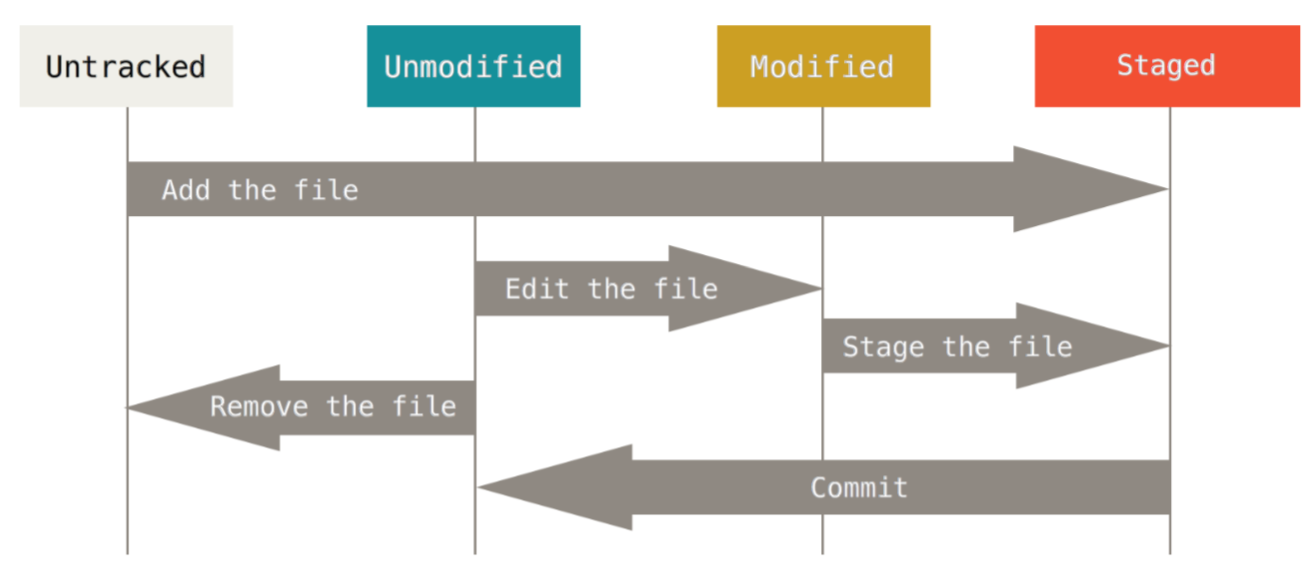
\includegraphics[width=1\textwidth]{image.png}
    \label{fig:logo}
\end{figure}
\subsection{Présentation du jeu}
\subsection{Direction artistique}
\subsection{Fonctionnalités}
\section{Organisation}
\subsection{}
\subsection{Sous partie 2}
\section{Partie 2-Les tableaux en Latex}

    Les algorithmes de \LaTeX pour mettre en forme les tableaux ont quelques imperfections. L’une d’entre elles est qu’il n’affiche pas automatiquement le texte sur plusieurs lignes dans les cellules, même si celui-ci déborde de la largeur de la page. Pour les colonnes qui contiendront une certaine quantité de texte, il est recommandé d’employer l’attribut p et d’indiquer la largeur désirée de la colonne (bien que cela puisse obliger à effectuer quelques ajustements avant d’obtenir le résultat souhaité) (figure2etfigure3oufigure 4)[3] [3]. ...

    Afin de mener à bien ce projet, nous avons suivi un planning prévisionnel qui nous a permis de nous organiser et de nous assurer que nous respections les dates limites. Nous avons donc dû faire un diagramme de Gantt pour nous aider à planifier nos tâches.
    \begin{figure}[h]
        \centering
        
\includegraphics[width=0.8\textwidth]{../../assets/Title Screen/BG.jpg}
        \label{fig:GANTT}
        \caption{Diagramme de Gantt}
    \end{figure}
\subsection{Planning Prévisionnel}
\begin{table}[h]
    \centering
    \begin{tabular}{|c|c|c|}
        \hline
        Un titre de colonne & Un autre titre & Encore un \\
        \hline
        à gauche & au centre & à droite \\
        \hline
        d & au centre & à droite \\
        \hline
        Si j’écris plus de texte je dépasse la taille de la page & texte & texte \\
        \hline
    \end{tabular}
    \vspace{1cm}
    \caption{\emph{Un tableau simple}}
    \label{tab:test}
\end{table}

\subsection{Répartition des tâches}
\subsection{Outils}
\newpage
\begin{center}
\begin{tabular}{|c|p{8cm}|}
\hline
2 - 1 & On met un grand texte qui sera sur plusieurs lignes \\
\hline
\end{tabular}
\end{center}

\section{Developpement}
\subsection{Gestions des ICMons}
    \subsubsection{structures de données}
    \subsubsection{systèmes de combats}

\subsection{Gestion des bases de données}
    \subsubsection{sauvegarde}
    \subsubsection{base de données des icmons}

\subsection{Gestion de la map}
    \subsubsection{chargement de la map}
    \subsubsection{caméra}
    \subsubsection{deplacement}

\subsection{rendu du jeu}
    \subsubsection{gestion de l'interface}
    \subsubsection{gestion des combats avec SDL}


\section{Bilan et résultats}
\section{Références}
\section{Annexes}
\end{document}